\documentclass[10pt,a4paper,notitlepage]{article}
\usepackage[utf8]{inputenc}
\usepackage{amsmath}
\usepackage{amsfonts}
\usepackage{amssymb}
\usepackage{fullpage}
\usepackage{lastpage}
\usepackage{lscape}
\usepackage{fancyhdr}
\usepackage{multirow}
\usepackage{fancyvrb}
\usepackage{xcolor}
\usepackage{tikz}
\usetikzlibrary{automata, positioning, arrows}
\usepackage{graphicx}
\graphicspath{{./Graphics/}}
\usepackage{float}
\usepackage{nameref}
\usepackage[backend=bibtex,style=authortitle-ibid]{biblatex}
\usepackage{diagbox}
\addbibresource{References.bib}
  
\author{Jonah Gibbon}

\pagestyle{fancy}
\fancyhf{}
\renewcommand{\headrulewidth}{0pt}
\cfoot{Page \thepage\ of \pageref{LastPage}}

\newcommand{\abs}[1]{\lvert#1\rvert}
\newcommand{\Z}{\mathbb{Z}}
\newcommand{\Q}{\mathbb{Q}}
\newcommand{\C}{\mathbb{C}}
\newcommand{\N}{\mathbb{N}}
\newcommand{\R}{\mathbb{R}}

\begin{document}

\subsection*{\centering Question 1}
In order to count the number of possible $(n,k)$-DFAs, we first examine a single state with alphabet $k$. Each letter can be directed to all $n$ states, so there are $n$ options for a single letter, and so $n^{k}$ for the complete alphabet. This applies to each state, so there are $n^{nk}$ ways of transitioning between each state. Each state can be an accepting or rejecting state, which can be chosen in a total of $2^{n}$ ways. We therefore conclude that the total number of $(n,k)$-DFAs is 
\begin{equation}
2^{n}\times n^{nk}
\end{equation}
Note this is the same number of different $n\times (k+1)$ transition tables, where the $(k+1)$th column can only equal 0 or 1, and the first $k$ columns can take $n$ different values.  The number of $(n,k)$-DFAs for $1\leq n\leq 6$ and $1\leq k\leq 4$ was calculated by \nameref{cd:1}, referenced on page \pageref{cd:1}, and are tabulated below in Table \ref{tb:1}. Note these values have been rounded to 2 significant figures.
\begin{table}[H]
\centering
\begin{tabular}{|c|cccc|} 
\hline  
\backslashbox[10mm]{$n$}{$k$} & 1 & 2 & 3 & 4\\
\hline 
1 & 2 & 2 & 2 & 2\\ 
2 & 16 & 64 & 260 & 1.0e+3\\ 
3 & 220 & 5.8e+3 & 1.6e+5 & 4.3e+6\\ 
4 & 4.1e+3 & 1.0e+6 & 2.7e+8 & 6.9e+10\\ 
5 & 1.0e+5 & 3.1e+8 & 9.8e+11 & 3.1e+15\\ 
6 & 3.0e+6 & 1.4e+11 & 6.5e+15 & 3.0e+20\\ \hline 
\end{tabular}
\caption{Number of $(n,k)$-DFAs}\label{tb:1}
\end{table}
Notice that these numbers grow large quickly, however many of these will be equivalent. We can also see that the number of $(1,k)$-DFAs is always 2. This makes sense, since all transitions must lead back to the start state. Therefore there are only ever two $(1,k)$-DFAs; one that accepts all inputs, and one that accepts none.

\subsection*{\centering Question 2}
\nameref{cd:2}, referenced on page \pageref{cd:2}, was used to determine the accessible states of DFA from it's transition table.\footnote{The functions \texttt{Accessible} and \texttt{Clean} defined in \nameref{cd:2} will be used implicitly throughout the rest of this project, and will no longer be included in any subsequent referencing.} The results calculated from the tables on the CATAM website are listed below.
\begin{table}[H]
\centering
\begin{tabular}{c|c|c}
Table Name & List of Accessible States & Fraction of Accessible States\\
\hline
\texttt{Table 1} &  1     2     3     5     6     9    10 & 7/10\\
\texttt{Table 2} & 1     2     3     4     5     6     7 & 7/7\\
\texttt{Table 3} & 1     2     3     4     5     6     7     8     9 & 9/9\\
\texttt{Table 4} & Too large to list & 76/100\\
\end{tabular}
\caption{List of Accessible States for Online Transition Tables}
\end{table}
The complexity of this algorithm is bounded by $O(kn)$. The code creates a 'queue' of states to examine which further states can be reached from them, as well as a $1\times n$ vector of accessible states that acts as a hash table for efficient indexing. For each state in the queue, the $k$ letters are applied to it, and all states reached are tested to see if they've been already declared accessible. This process takes $O(1)$ operations, and since this happens for each letter, and then for each element in the queue (which has length bounded by $n$), the total number of operations is at most $O(kn)$.\\

\nameref{cd:3}, referenced on page \pageref{cd:3}, was used to generate all possible transition tables, and then remove the ones with inaccessible states.\footnote{The function \texttt{GenerateEverything} defined in \nameref{cd:3} will be used implicitly throughout the rest of this project, and will no longer be included in subsequent referencing.} Since states being accessible/inaccessible does not depend on whether they are accepting or not, the last column of the transition tables were not generated, increasing the efficiency of the code. Therefore the results calculated are out by a factor of $2^{n}$. Such results are tabulated below in Table \ref{tb:4}.
\begin{table}[H]
\centering
\begin{tabular}{c|c}
$n$ & Number of DFAs\\
\hline
1 & $1\times 2^{1}=2$\\
2 & $12\times 2^{2}=48$\\
3 & $432\times 2^{3}=3456$\\
4 & $31488\times 2^{4}=503808$
\end{tabular}
\caption{Number of $(n,2)$-DFAs with no inaccessible states}\label{tb:4}
\end{table}
\subsection*{\centering Question 3}
\nameref{cd:4}, referenced on page \pageref{cd:4}, was written to remove all inaccessible states from a transition table using the function \texttt{Clean}, then minimise the resultant table with Hopcroft's table filling algorithm using functions \texttt{Hopcroft} and \texttt{Minimise}.\footnote{The functions \texttt{Hopcroft} and \texttt{Minimise} will be used implicitly throughout the rest of this project, and will no longer be included in subsequent referencing.} The results of minimising the transition tables on the CATAM website are tabulated below in Table \ref{tb:5}.

\begin{table}[H]
\centering
\begin{tabular}{c|c|c}
 \texttt{Table 1} & \texttt{Table 2} &  \texttt{Table 3}\\ \hline 
$\begin{array}{|ccc|}
\hline
2 & 4 & 1\\ 6 & 6 & 1\\ 1 & 2 & 0\\ 5 & 2 & 0\\ 3 & 4 & 0\\ 5 & 2 & 1\\ \hline\end{array}$  & $
\begin{array}{|cccc|}\hline 2 & 2 & 2 & 1\\ 2 & 2 & 2 & 0\\ \hline \end{array}$ &  $\begin{array}{|cccc|}  9 & 5 & 5 & 1\\ 7 & 2 & 6 & 0\\ 7 & 4 & 1 & 0\\ 1 & 2 & 8 & 0\\ 8 & 1 & 6 & 0\\ 9 & 9 & 8 & 0\\ 9 & 3 & 4 & 0\\ 8 & 3 & 5 & 0\\ 8 & 3 & 1 & 0\\ \hline \end{array}$ \\ 
\end{tabular}
\caption{Minimisation of Online Transition Tables}\label{tb:5}
\end{table}

We see that the first DFA has one pair of equivalent states, since its transition table has one less state than in Question 2. It's interesting to see that \texttt{Table 2} minimises to a very small DFA, even if all it's states were accessible. \texttt{Table 3} is already minimal, since it has not been reduced and has its original states.\\

The complexity of the table filling algorithm is $O(n^{2}k)$. It initially starts by running through each pair of states and marking their position in the table if one is accepting and the other rejecting ($O(n^{2})$). It proceeds to calculate and store the values of $\delta(p,a),\delta(q,a)$, for all pairs of states $p,q$ and all $a$ in the alphabet ($O(n^{2}k)$). From this information, we can iterate backwards through this list of all transitions to marked pairs. This list will be bounded by size $O(n^{2}k)$, and so we conclude that this table filling algorithm is $O(n^{2}k)$. Note there are faster known algorithms, such as Hopcrofts Algorithm, which uses the refinement of partitions of states into equivalence classes, which converges to the equivalent states. This algorithm has worst case complexity $O(kn\log(n))$.

To update the transition table takes a further $O(n^{2}k)$ operations. For each pair of equivalent states, the algorithm removes the one from the lower row and redirects transitions to the other state. This will take $O(nk)$ iterations through the transition table, and so in total $O(n^{2}k)$.

\subsection*{\centering Question 4}
In order to calculate the number of unique regular languages definable by a minimal $(n,k)$-DFA, it suffices to count how many unique minimal DFAs there are, since each define a unique language. We use the results from Question 2, by starting with all possible transition tables and removing the ones with inaccessible states (since they cannot define a minimal DFA). By accounting for all possible combinations of accept states to this set, we then iterate through those remaining, removing ones that minimise to a DFA with strictly smaller states. These DFAs now remaining are all possible minimal $(n,k)$-DFAs. We know that a minimal DFA is unique up to a reordering of states, and since we assume state 1 to be fixed as the starting state, there are $(n-1)!$ ways of doing this. Therefore the results published by \nameref{cd:5}, referenced on page \pageref{cd:5}, and which implements the procedure described above, will be out by this factor, and so the code corrects for this. The results are tabulated below in Table \ref{tb:6}.
\begin{table}[H]
\centering
\begin{tabular}{c|c}
$n$ & Number of Languages\\
\hline 1 & $2/1=2$\\
2 & $24/1=24$ \\
3 & $2056/2=1028$\\
4 & $336084/6=56014$
\end{tabular}
\caption{Number of distinct regular languages for an $(n,2)$-DFA}\label{tb:6}
\end{table}
\subsection*{\centering Question 5}
This result is a direct consequence of the pumping lemma. Suppose $\mathcal{L}(D)$ contained a word $w$ of length $n\leq \abs{w}$. Then since $n$ will always be greater than the pumping length $L$ (since by the pigeon-hole principle the word's path within the DFA's transition diagram must visit a state at least twice), we may apply the lemma, so there exist words $x,y,z$ where $w=xyz$ such that $\abs{y}>0$ $\abs{xy}\leq n$ and for each $i\geq 0$, $xy^{i}z\in \mathcal{L}(D)$. Therefore $\abs{\mathcal{L}(D)}$ is infinite.

Conversely if $\abs{\mathcal{L}(D)}$ is infinite, start with a word $w_{1}$ such that we may apply the pumping lemma. Then pump down (set $i=0$ in the above) to find a new word of strictly smaller length $w_{2}=xz$. We argue that the size of $y$ is at most $n$, since this is the largest possible 'loop' within the words path which does not contain smaller loops. Therefore the length of $w_{2}$ will have decreased at most length $n$. By induction, we repeat the above until $\abs{w_{n}}<n$. However before this occurs, we will have found a word $w_{i}\in \mathcal{L}(D)$ with a length between $n\leq \abs{w_{i}}\leq 2n-1$. Hence the reverse implication holds true and we're done.

\subsection*{\centering Question 6}
\nameref{cd:6}, referenced on page \pageref{cd:6}, was used to calculate the sizes of the languages defined by the tables on the CATAM website.\footnote{The functions \texttt{GenerateWords} and \texttt{runWord} defined in \nameref{cd:6} will be used implicitly throughout the rest of the project, and won't be included in any subsequent referencing.} The results are published below in Table \ref{tb:2}:
\begin{table}[H]
\centering
\begin{tabular}{c|c|c}
Table Name & $\abs{\mathcal{L}(D)}$ & Word $w$ with $\abs{w}\geq n$ (if it exists) \\ \hline
\texttt{Table 1} & $\infty$ & 111111\\
\texttt{Table 2} & 1 & $\ast$\\
\texttt{Table 3} & $\infty$ & 111111221\\
\end{tabular}
\caption{$\abs{\mathcal{L}(D)}$ for Online Transition Tables}\label{tb:2}
\end{table}
The method behind this algorithm is to first determine if the language is infinite, by trying each possible word of length $n\leq \abs{w}\leq 2n-1$, and seeing if any of them are accepted. If they are, by Question 5 we may stop and claim that this language is indeed infinite. This involves testing $O(k^{2n})$ different words, meaning this algorithm runs exponentially in $n$, however for the sizes of $n$ and $k$ given in the examples this does not majorly affect us. If we cannot find such a word, then the algorithm iterates through each word where $0\leq \abs{w} <n$ and counts the size of the language. 

It is crucial the transition tables are minimised before this algorithm runs, since by reducing the value of $n$, we seriously reduce the number of words we must test. Taking \texttt{Table 1} as an example, if we hadn't minimised it, we would have to test roughly 260 times more words than if we had. However we only need to find a word of length 6 to prove the language in infinite, instead of a word of length 10.

\subsection*{\centering Question 7}
\nameref{cd:7}, referenced on page \pageref{cd:7}, was used to calculate $f(n,2,s)$ for $1\leq n\leq 4$ and $0\leq s\leq 2^{n}-1$. Note the results published below in Table \ref{tb:3} have been altered by the factor of $(n-1)!$, justified at the end of Question 4.

\begin{table}[H]
\centering
\begin{tabular}{c|cccccccccccccccc}
 $s$ & 0 & 1 & 2 & 3 & 4 & 5 & 6 & 7 & 8 & 9 & 10 & 11 & 12 & 13 & 14 & 15\\ 
\hline $f(1,k,s)$ & 1 & 0\\
 $f(2,2,s)$ & 0 & 1 & 0 & 0\\
 $ f(3,2,s)$ & 0 & 2 & 3 & 1 & 0 & 0 & 0 & 0\\
 $f(4,2,s)$ & 0 & 4 & 16 & 20 & 13 & 5 & 1 & 1 & 0 & 0 & 0 & 0 & 0 & 0 & 0 & 0\\ 
\end{tabular}
\caption{Value of $f(n,2,s)$ for $0\leq s\leq 2^{n}-1$}\label{tb:3}
\end{table}
The blank space represent zeros, since if $s\geq 2^{n}$, then by a counting argument, there must be at least one word in this language that has length of at least $n$. But then this language is infinite (Question 5), and hence $f(n,2,s)=0$ for all $s\geq 2^{n}$. It appears that $f(n,2,s)=0$ for all $s\geq 2^{n-1}$, and this will be discussed further in Question 9, on page \pageref{sc:9}. It's interesting to see how small the proportion of finite languages there are.
\subsection*{\centering Question 8}
Below are the minimal $(n, 2)$-transition tables when $s$ equals 1 or $2^{n-1}-1$.
\begin{table}[H]
\centering
\begin{tabular}{|c|c|c|}
\hline
$s$ & Transition Table & $\mathcal{L}(D)$ \\
\hline
$0$ & $\begin{array}{ccc}  1 & 1 & 0  \end{array}$ & $ \emptyset $\\ \hline
\end{tabular}
\caption{$(1,2)$-transition tables}
\end{table}

\begin{table}[H]
\centering
\begin{tabular}{|c|c|c|}\hline
$s$ & Transition Table & $\mathcal{L}(D)$ \\
\hline
$1$ & $\begin{array}{ccc} 2 & 2 & 1\\ 2 & 2 & 0 \end{array}$ & $\lbrace \epsilon \rbrace$\\ \hline
\end{tabular}
\caption{$(2,2)$-transition tables}
\end{table}

\begin{table}[H]
\centering
\begin{tabular}{|c|c|c|} \hline
$s$ & Transition Table & $\mathcal{L}(D)$ \\
\hline
$1$ & $\begin{array}{ccc} 2 & 3 & 0\\ 3 & 3 & 1\\ 3 & 3 & 0 \end{array}$ & $\lbrace 1 \rbrace$\\ \hline 
$1$ & $\begin{array}{ccc} 3 & 2 & 0\\ 3 & 3 & 1\\ 3 & 3 & 0 \end{array}$ & $\lbrace 2 \rbrace$\\ \hline
$3$ & $\begin{array}{ccc} 2 & 2 & 1\\ 3 & 3 & 1\\ 3 & 3 & 0 \end{array}$ & $\lbrace \epsilon, 1 ,2\rbrace$\\ \hline
\end{tabular}
\caption{$(3,2)$-transition tables}
\end{table}

\begin{table}[H]
\centering
\begin{tabular}{|c|c|c|}\hline
$s$ & Transition Table & $\mathcal{L}(D)$ \\
\hline
$1$ & $\begin{array}{ccc} 4 & 3 & 0\\ 3 & 3 & 1\\ 3 & 3 & 0\\ 2 & 3 & 0 \end{array}$ & $\lbrace 11\rbrace$\\ \hline
$1$ & $\begin{array}{ccc} 4 & 3 & 0\\ 3 & 3 & 1\\ 3 & 3 & 0\\ 3 & 2 & 0 \end{array}$ & $\lbrace 12 \rbrace$\\ \hline 
$1$ & $\begin{array}{ccc} 3 & 4 & 0\\ 3 & 3 & 1\\ 3 & 3 & 0\\ 2 & 3 & 0 \end{array}$ & $\lbrace  21\rbrace$\\ \hline
$1$ & $\begin{array}{ccc} 3 & 4 & 0\\ 3 & 3 & 1\\ 3 & 3 & 0\\ 3 & 2 & 0 \end{array}$ & $\lbrace 22 \rbrace$\\ \hline
$7$ & $\begin{array}{ccc} 2& 2 & 1\\ 3 & 3 & 1\\ 4 & 4 & 1\\ 4 & 4 & 0 \end{array}$ & $\lbrace \epsilon,1,2,11,12,21,22 \rbrace$\\ \hline
\end{tabular}
\caption{$(4,2)$-transition tables}
\end{table}
\nameref{cd:7} was altered to narrow down the transition tables to check, by displaying the ones that define finite languages when $s=1$ or $2^{n-1}-1$. The following code was added at line 80:
\begin{verbatim}
if LanguageSize==1
        disp('LanguageSize=1')
        disp(MinimalDFAs{SuperCounter,1})
        disp(latex(sym(MinimalDFAs{SuperCounter,1})))
        disp('*****')
end
if LanguageSize==2^(n-1)-1
        disp('LanguageSize=2^(n-1)-1')
        disp(MinimalDFAs{SuperCounter,1})
        disp(latex(sym(MinimalDFAs{SuperCounter,1})))
        disp('*****')
end
\end{verbatim}
The outputted tables were then gone through by hand to remove the equivalent ones. 

Observe that for $n\geq 2$, the languages of size $1$ seem to consist of all $n-2$ length words, and the languages of size $2^{n-1}-1$ consist of all words of size less than or equal to $n-2$. This will be discussed further in Question 9.
\subsection*{\centering Question 9}\label{sc:9}
To begin this question, we first address the case when $2^{n-1}\leq s\leq 2^{n}-1$. Should a language exist of this size, then by a counting argument there exists an accepting word of length at least $n-1$. This word cannot be at least length $n$, otherwise by Question 5 the language would be infinite. We deduce that this language contains a word of exact length $n-1$.\\

We claim that any language that contains a word $w=w_{1}\hdots w_{n-1}$ of length $n-1$ on a DFA with $n$ states must be infinite. For a contradiction, suppose that this language was finite. Then the 'path' this word takes in the DFA must not visit a state more than once, since otherwise we could pump this loop up to create an infinite language. We therefore deduce that this word will visit each state, before finishing in an accept state. The DFA will therefore be equivalent to the one in Figure \ref{fg:1}, up to reordering states, and that the states $1$ to $n-1$ may be a mixture of accept/reject states. 
\begin{figure}[H]
\centering
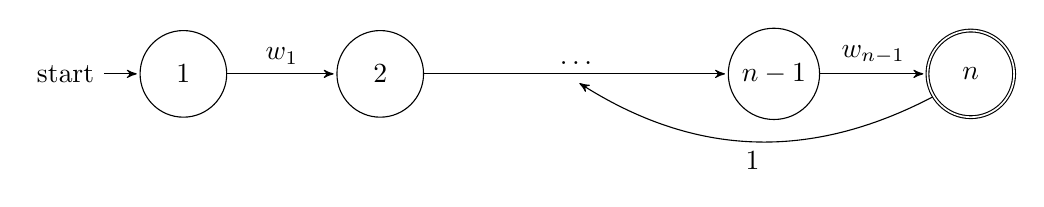
\begin{tikzpicture}[->,>=stealth', shorten >=1pt, align=center, state/.style={circle, draw, minimum size=1.1cm}]
\node[state, initial] at (-5,0)(q1) {$1$};
\node[state] at (-2.5,0) (q2) {$2$};
\node[state] at (2.5,0) (q3){$n-1$};
\node[state,accepting] at (5,0) (q4) {$n$};
\draw (q1) edge[above] node{$w_{1}$} (q2);
\draw (q2) edge[above] node{$\hdots$} (q3);
\draw (q3) edge[above] node{$w_{n-1}$} (q4);
\draw (q4) edge[bend left, below] node{$1$} (0,-0.1);
\end{tikzpicture}
\caption{DFA with accept word of length $n-1$}\label{fg:1}
\end{figure}
Suppose that the letter $1$ went to state $i$ from state $n$. Then we deduce that the word 
\begin{equation}
w\left(1w_{i}w_{i+1}\hdots w_{n-1}\right)^{k}\in\mathcal{L}(D)
\end{equation}
for all $k\in \N_{0}$, and hence the language is infinite. (Obviously if $i=n$ this language is also infinite). We have therefore proved that $f(n,2,s)=0$ for all $s\geq 2^{n-1}$. This explains the zeros that appear in these positions in Table \ref{tb:3}.\\

We will prove that
\begin{equation}
f(n,2,1)=\begin{cases}
      0 & \text{if $n=1$}\\
      2^{n-2} & \text{if $n\geq 2$}
    \end{cases}
\end{equation}
When $n=1$, the DFA will either accept all words or none at all, depending on if the start state is accepting or not. Because of this there will never be a language of size 1. When $n\geq 2$, suppose the language $\mathcal{L}(D)$ consists of the single word $w=w_{1}\hdots w_{n-2}$ of length $n-2$. This language can be represented by the minimal $(n,2)$-DFA in Figure \ref{fg:2}.
\begin{figure}[H]
\centering
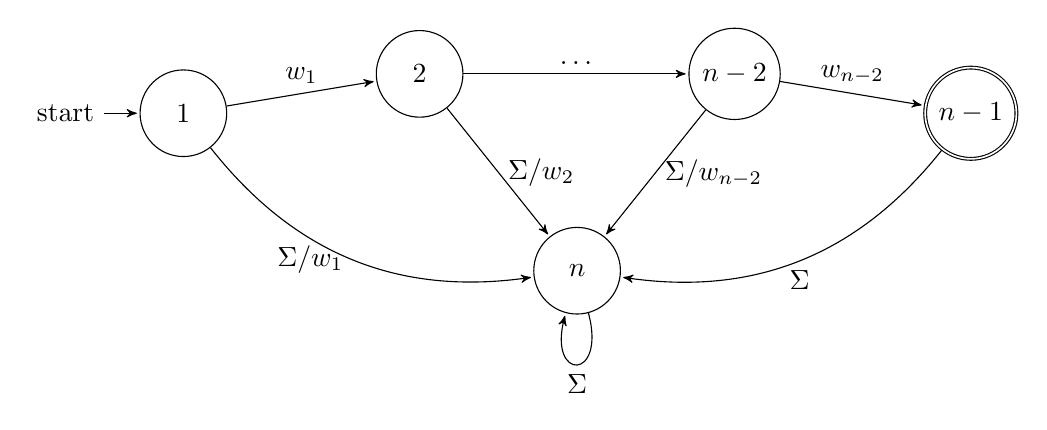
\begin{tikzpicture}[->,>=stealth', shorten >=1pt, align=center, state/.style={circle, draw, minimum size=1.1cm}]
\node[state, initial] at (-5,0)(q1) {$1$};
\node[state] at (-2,0.5) (q2) {$2$};
\node[state] at (2,0.5) (q3){$n-2$};
\node[state,accepting] at (5,0) (q4) {$n-1$};
\node[state] at (0,-2) (q5) {$n$};
\draw (q1) edge[above] node{$w_{1}$} (q2);
\draw (q2) edge[above] node{$\hdots$} (q3);
\draw (q3) edge[above] node{$w_{n-2}$} (q4);
\draw (q4) edge[bend left, below] node{$\Sigma$} (q5);
\draw (q5) edge[loop below] node{$\Sigma$} (q5);
\draw (q3) edge[right] node{$\Sigma /w_{n-2}$} (q5);
\draw (q2) edge[right] node{$\Sigma /w_{2}$} (q5);
\draw (q1) edge[bend right, left] node{$\Sigma /w_{1}$} (q5);
\end{tikzpicture}
\caption{Minimal $(n,2)$-DFA with $\abs{\mathcal{L}(D)}=1$}\label{fg:2}
\end{figure}
where $\Sigma=\lbrace 1,2\rbrace$.  This DFA is  minimal, since the pair of states $i,j>i$ where $j\neq n$ are distinguishable by the word $w_{j}w_{j+1}\hdots w_{n-2} \, \epsilon$, and when $j=n$ by $w_{i}w_{i+1}\hdots w_{n-2}\, \epsilon $. We will now rely on the theorem that a language can only be represented by a unique minimal DFA (up to a reordering of states), and since there are $2^{n-2}$ words of length $n-2$, $f(n,2,1)= 2^{n-2}$.\\

We will also prove that
\begin{equation}
f(n,2,2^{n-1}-1)=1
\end{equation}
for all $n$. From a counting argument, this language must be the set of all words of length $n-2$ or less, otherwise it would contain a word $w$ with $\abs{w}\geq n-1$, and hence the language would be infinite. Now that this language is exactly specified, it remains to show that it is accepted by a minimal $(n,2)$-DFA. This is not difficult, since the following DFA in Figure \ref{fg:3} does exactly that.
\begin{figure}[H]
\centering
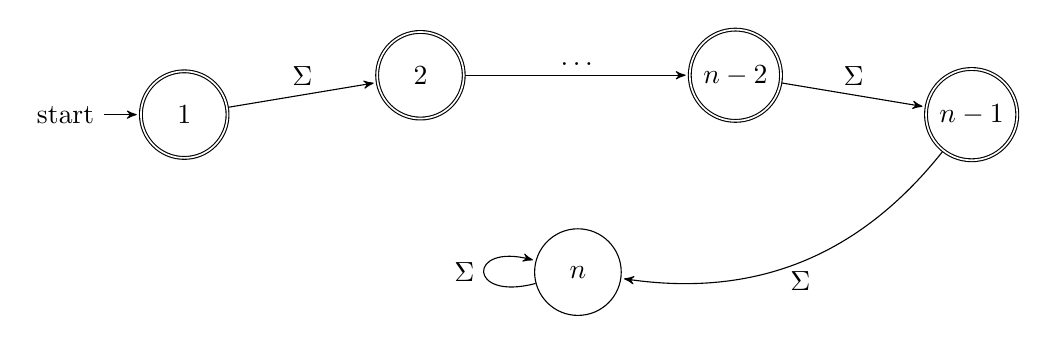
\begin{tikzpicture}[->,>=stealth', shorten >=1pt, align=center, state/.style={circle, draw, minimum size=1.1cm}]
\node[state, initial,accepting] at (-5,0)(q1) {$1$};
\node[state,accepting] at (-2,0.5) (q2) {$2$};
\node[state,accepting] at (2,0.5) (q3){$n-2$};
\node[state,accepting] at (5,0) (q4) {$n-1$};
\node[state] at (0,-2) (q5) {$n$};
\draw (q1) edge[above] node{$\Sigma$} (q2);
\draw (q2) edge[above] node{$\hdots$} (q3);
\draw (q3) edge[above] node{$\Sigma$} (q4);
\draw (q4) edge[bend left, below] node{$\Sigma$} (q5);
\draw (q5) edge[loop left] node{$\Sigma$} (q5);
\end{tikzpicture}
\caption{Minimal $(n,2)$-DFA with $\abs{\mathcal{L}(D)}=2^{n-1}-1$}\label{fg:3}
\end{figure}
This DFA is indeed minimal, since each pair of states $i,j>i$ can be distinguished by the word $11\hdots 1$ (where there are $n-j$ 1s). Hence $f(n,2,2^{n-1}-1)=1$. Note this proof is only valid for $n\geq 2$, however the case with $n=1$ is trivial, and can be verified that it still fits this formula.

Both these closed form expressions hold for the examples calculated in Table \ref{tb:3}.


\pagebreak
\section*{\centering Code}
\subsection*{\centering Code 1}\label{cd:1}
\begin{verbatim}
Count=1;
digits(10)
Data=zeros(4,6);
while Count<=6
    SubCount=1;
    while SubCount<=4
        Data(SubCount,Count)=2^Count * Count^(Count*SubCount);
        SubCount=SubCount+1;
    end
    Count=Count+1;
end
disp(Data')
latex(sym(vpa(Data')))
\end{verbatim}
\pagebreak

\subsection*{\centering Code 2}\label{cd:2}
\begin{verbatim}
TransTab=[
2 5 1
10 10 1
1 2 0
8 3 0
9 2 0
9 2 0
1 9 1
4 6 0
3 6 0
9 2 1];
n=size(TransTab,1);
k=size(TransTab,2)-1;

m=Accessible(TransTab,n,k)
sum(m(:,2))

function [TransTab,n] = Clean(TransTab,n,k)
AccessibleStates=Accessible(TransTab,n,k);
ChopCount=0;
Counter=1;
while Counter<=n
    if AccessibleStates(Counter,2)==0
        TransTab(Counter-ChopCount,:)=[];
        SubCounter=1;
        while SubCounter<=n-ChopCount-1
            Sub2Counter=1;
            while Sub2Counter<=k
                if TransTab(SubCounter,Sub2Counter)>Counter-ChopCount
                    TransTab(SubCounter,Sub2Counter)=TransTab(SubCounter,Sub2Counter)-1;
                end
                Sub2Counter=Sub2Counter+1;
            end
            SubCounter=SubCounter+1;
        end
        ChopCount=ChopCount+1;
    end
    Counter=Counter+1;
end
n=n-ChopCount;
end

function AccessibleStates = Accessible(TransTab,n,k)
Queue=zeros(1,n);
Queue(1,1)=1;
LengthQueue=1;
Counter=1;
AccessibleStates=zeros(n,2);
AccessibleStates(:,1)=1:n;
AccessibleStates(1,2)=1;

while Counter<=LengthQueue
    SubCounter=1;
    while SubCounter<=k
        Element=TransTab(Queue(Counter),SubCounter);
        if AccessibleStates(Element,2)==0
            AccessibleStates(Element,2)=1;
            Queue(LengthQueue+1)=Element;
            LengthQueue=LengthQueue+1;
        end
        SubCounter=SubCounter+1;
    end
    Counter=Counter+1;
end
end
\end{verbatim}
\pagebreak

\subsection*{\centering Code 3}\label{cd:3}
\begin{verbatim}
n=4;
k=2;
Everything=GenerateEverything(n,k);
disp(size(Everything,1))

function TransitionTables = GenerateEverything(n,k)
States=(1:n)';
Fill=cell(1,k);
Counter=1;
while Counter<=k
    Fill{1,Counter}=States;
    Counter=Counter+1;
end
Filler=Fill;
[Filler{:}] = ndgrid(Fill{:});
Bank=cell2mat(cellfun(@(m)m(:),Filler,'uni',0));
BankSize=size(Bank,1);

States=(1:BankSize)';
Fill=cell(1,n);
Counter=1;
while Counter<=n
    Fill{1,Counter}=States;
    Counter=Counter+1;
end
Filler=Fill;
[Filler{:}] = ndgrid(Fill{:});
TableIndex=cell2mat(cellfun(@(m)m(:),Filler,'uni',0));
Counter=1;
TransitionTables=cell(0,1);
Tally=0;
while Counter<=size(TableIndex,1)
    Table=zeros(n,k);
    SubCounter=1;
    while SubCounter<=n
        Table(SubCounter,:)=Bank(TableIndex(Counter,SubCounter),:);
        SubCounter=SubCounter+1;
    end
    M=Accessible(Table,n,k);
    if sum(M(:,2))==n
        Tally=Tally+1;
        TransitionTables{Tally,1}=Table;
    end
    Counter=Counter+1;
end
end
\end{verbatim}
\pagebreak

\subsection*{\centering Code 4}\label{cd:4}
\begin{verbatim}
TransTab=[
    2 5 1
10 10 1
1 2 0
8 3 0
9 2 0
9 2 0
1 9 1
4 6 0
3 6 0
9 2 1
    ];
n=size(TransTab,1);
k=size(TransTab,2)-1;

tic
[TransTab,n]=Clean(TransTab,n,k)
[TransTab,n]=Minimise(TransTab,n,k)
toc

function [TransTab,n] = Minimise(TransTab,n,k)
HopTable=Hopcroft(TransTab,n,k);
SubCounter=n;
while SubCounter>1
    Counter=1;
    while Counter<=SubCounter-1
        if HopTable(SubCounter,Counter)==0
            Sub2Counter=1;
            while Sub2Counter<=k
                 Sub3Counter=1;
                 while Sub3Counter<=n
                     if TransTab(Sub3Counter,Sub2Counter)==SubCounter
                         TransTab(Sub3Counter,Sub2Counter)=Counter;
                     end
                     Sub3Counter=Sub3Counter+1;
                 end
                 Sub2Counter=Sub2Counter+1;
            end
        end
        Counter=Counter+1;
    end
    SubCounter=SubCounter-1;
end
TransTab=Clean(TransTab,n,k);
n=size(TransTab,1);
end

function HopTable = Hopcroft(TransTab,n,k)
HopTable=zeros(n,n);
Queue=zeros(0,2);
Counter=1;
while Counter<=n-1
    SubCounter=Counter+1;
    while SubCounter<=n
        if TransTab(SubCounter,k+1)~=TransTab(Counter,k+1)
            HopTable(SubCounter,Counter)=1;
            Queue=[Queue; SubCounter,Counter];
        end
        SubCounter=SubCounter+1;
    end
    Counter=Counter+1;
end
Lists=cell(n,n);
Counter=1;
while Counter<=n-1
    SubCounter=1+Counter;
    while SubCounter<=n
        if HopTable(SubCounter,Counter)==0
            Sub2Counter=1;
            while Sub2Counter<=k
                XState=TransTab(SubCounter,Sub2Counter);
                YState=TransTab(Counter,Sub2Counter);
                if XState==YState
                else
                    if XState<YState
                    else
                        Z=YState;
                        YState=XState;
                        XState=Z;
                    end
                    Lists{YState,XState}=[Lists{YState,XState}; SubCounter,Counter];
                end
                Sub2Counter=Sub2Counter+1;
            end
        end
        SubCounter=SubCounter+1;
    end
    Counter=Counter+1;
end
QueueLength=size(Queue,1);
Counter=1;
while Counter<=QueueLength
    CurrentList=Lists{Queue(Counter,1),Queue(Counter,2)};
    SubCounter=1;
    while SubCounter<=size(CurrentList,1)
        if HopTable(CurrentList(SubCounter,1),CurrentList(SubCounter,2))==0
            HopTable(CurrentList(SubCounter,1),CurrentList(SubCounter,2))=1;
            Queue=[Queue;CurrentList(SubCounter,:)];
            QueueLength=QueueLength+1;
        end
        SubCounter=SubCounter+1;
    end
    Counter=Counter+1;
end
end
\end{verbatim}
\pagebreak

\subsection*{\centering Code 5}\label{cd:5}
\begin{verbatim}
n=3;
k=2;

tic
Everything=GenerateEverything(n,k);
States=(0:1)';
Fill=cell(1,n);
Counter=1;
while Counter<=n
    Fill{1,Counter}=States;
    Counter=Counter+1;
end
Filler=Fill;
[Filler{:}] = ndgrid(Fill{:});
Bank=cell2mat(cellfun(@(m)m(:),Filler,'uni',0));

Fill=cell(1,2);
Fill{1,1}=(1:size(Everything,1))';
Fill{1,2}=(1:size(Bank,1))';
Filler=Fill;
[Filler{:}] = ndgrid(Fill{:});
TableIndex=cell2mat(cellfun(@(m)m(:),Filler,'uni',0));


MinimalDFAs=cell(0,1);
Tally=0;
Counter=1;
while Counter<=size(TableIndex,1)
    Table=[Everything{TableIndex(Counter,1),1} Bank(TableIndex(Counter,2),:)'];
    [Table,TabSize]=Minimise(Table,n,k);
    if TabSize==n
        Tally=Tally+1;
        MinimalDFAs{Tally,1}=Table;
    end
    Counter=Counter+1;
end
disp('Number of unique languages:')
disp(size(MinimalDFAs,1)/factorial(n-1))
toc
\end{verbatim}
\pagebreak

\subsection*{\centering Code 6}\label{cd:6}
\begin{verbatim}
TransTab=[
    2 5 1
10 10 1
1 2 0
8 3 0
9 2 0
9 2 0
1 9 1
4 6 0
3 6 0
9 2 1
    ];
n=size(TransTab,1);
k=size(TransTab,2)-1;
[TransTab,n]=Minimise(TransTab,n,k);

Length=n;
Flag=0;
while Length<=n
    Words=GenerateWords(Length,k);
    Counter=1;
    while Counter<=k^Length
        if runWord(TransTab,Words(Counter,:),k)==1
            disp('Language Infinite')
            disp('Word')
            disp(Words(Counter,:))
            Flag=1;
            break
        end
        Counter=Counter+1;
    end
    Length=Length+1;
    if Flag==1
        break
    end
end
if Flag==0
    disp('Language Finite')
    if TransTab(1,k+1)==1
        LanguageSize=1;
    else
        LanguageSize=0;
    end
    Length=1;
    while Length<=n-1
        Words=GenerateWords(Length,k);
        Counter=1;
        while Counter<=k^Length
            if runWord(TransTab,Words(Counter,:),k)==1
                LanguageSize=LanguageSize+1;
            end
            Counter=Counter+1;
        end
        Length=Length+1;
    end
    fprintf('Size: %d \n',LanguageSize)
end

function answer = GenerateWords(Length,k)
States=(1:k)';
Fill=cell(1,Length);
Counter=1;
while Counter<=Length
    Fill{1,Counter}=States;
    Counter=Counter+1;
end
Filler=Fill;
[Filler{:}] = ndgrid(Fill{:});
answer=cell2mat(cellfun(@(m)m(:),Filler,'uni',0));
end


function verdict = runWord(TransTab,Word,k)
    Length=size(Word,2);
    Counter=1;
    State=1;
    while Counter<=Length
        State=TransTab(State,Word(1,Counter));
        Counter=Counter+1;
    end
    verdict=TransTab(State,k+1);
end
\end{verbatim}
\pagebreak

\subsection*{\centering Code 7}\label{cd:7}
\begin{verbatim}
n=2;
k=2;

tic
Everything=GenerateEverything(n,k);
States=(0:1)';
Fill=cell(1,n);
Counter=1;
while Counter<=n
    Fill{1,Counter}=States;
    Counter=Counter+1;
end
Filler=Fill;
[Filler{:}] = ndgrid(Fill{:});
Bank=cell2mat(cellfun(@(m)m(:),Filler,'uni',0));

Fill=cell(1,2);
Fill{1,1}=(1:size(Everything,1))';
Fill{1,2}=(1:size(Bank,1))';
Filler=Fill;
[Filler{:}] = ndgrid(Fill{:});
TableIndex=cell2mat(cellfun(@(m)m(:),Filler,'uni',0));


MinimalDFAs=cell(0,1);
Tally=0;
Counter=1;
while Counter<=size(TableIndex,1)
    Table=[Everything{TableIndex(Counter,1),1} Bank(TableIndex(Counter,2),:)'];
    [Table,TabSize]=Minimise(Table,n,k);
    if TabSize==n
        Tally=Tally+1;
        MinimalDFAs{Tally,1}=Table;
    end
    Counter=Counter+1;
end


fData=zeros(2^n,2);
fData(:,1)=0:2^n-1;
SuperCounter=1;
while SuperCounter<=size(MinimalDFAs,1)
    lineLength=fprintf('Completion: %.1f%%',SuperCounter*100/size(MinimalDFAs,1));
    TransTab=MinimalDFAs{SuperCounter,1};
    Length=n;
    Flag=0;
    while Length<=2*n-1
        Words=GenerateWords(Length,k);
        Counter=1;
        while Counter<=k^Length
            if runWord(TransTab,Words(Counter,:),k)==1
                Flag=1;
                break
            end
            Counter=Counter+1;
        end
        Length=Length+1;
        if Flag==1
            break
        end
    end
    if Flag==0
        if TransTab(1,k+1)==1
            LanguageSize=1;
        else
            LanguageSize=0;
        end
        Length=1;
        while Length<=n-1
            Words=GenerateWords(Length,k);
            Counter=1;
            while Counter<=k^Length
                if runWord(TransTab,Words(Counter,:),k)==1
                    LanguageSize=LanguageSize+1;
                end
                Counter=Counter+1;
            end
            Length=Length+1;
        end
        fData(LanguageSize+1,2)=fData(LanguageSize+1,2)+1;
    end
    fprintf(repmat('\b',1,lineLength))
    SuperCounter=SuperCounter+1;
end
fData(:,2)=fData(:,2)./factorial(n-1);
disp(fData)
latex(sym(fData'))
toc
\end{verbatim}

\pagebreak
\end{document}
